%Notes:   
%Reason for assumption that mean of this distribution is the most likely the correct value, due to nature of the distributions. 
%scalar samples from vb is symmetrically weighted to both sides? interpretation?
%Possible influences on this deviation from the expected predictions: 
% absolute return value (higher returns get underestimated, lower returns get overestimated, leads to models with incorporated volatility, or broader flanks), 
% input data size (possible masking of data structure through sheer size, size prop. complexity of data structure in regime of N >= x1(???), possible data sizes not reflecting all structure due to missing inputs N<=x1, find optimum.), 
% choice of data (randomized stocks, structured stocks by ressort, structured stocks by alphabet in company name list) and observed pros and cons of these choices, 
% number of observed days for training (influence of training days and influence of how the progression of time influences prediction accuracy), 
% influence of hyperparameters (kernel lengthscale prop. to flexibility of change in single function draws from function space, function noise as prop. to self correlation since only added to diagonal, influence of jitter for numerical stability, influence of kernel noise prop. to e.g. volatility as it is unique to every stock (even though it is observed only during once)), 
% influence of latent positions/correlations (how does the grouping change with N-size, D-size) and 
% sampler ELBO convergence (should the convergence ratio be chosen smaller to definitely land in a minimum, should sampler do more runs because differences between found minima is large, etc.). 
% PLOTS Percentage of overpredicted and underpredicted stocks (in dependence of N-size, stock-groups, effect of stock groups rising and falling together (source???)). Influences of kernels, Qs. 

The Gaussian process latent variable model (GPLVM) is the basis of all following models. This stochastic process tries to learn a covariance structure from the data. All stocks are assigned a position in latent space, which influences the covariance structure the process can reproduce. This influences the covariance matrix, which is the key element of the learning equation of the GPLVM, representing the covariance structure learned. Data is fed into the model as a matrix of size $\mathbb{R}^{NxD}$, with $N$ stocks' returns observed over a timespan of $D$ days. If no data was available, the spot in the matrix was assumed to be 0, which is a reasonable assumption, since returns over small timespans are close to zero with only a small drift towards positive values. Then, the calculation specified by the model, as explained in more detail in the previous chapter \ref{sec:models}, is carried out. Samples from the Variational Bayes algorithm are generated and used to calculate the mean prediction for a specific entry of a matrix, vector, or simply a scalar. With these, the interpretation is carried out. 
\begin{figure}[h!]%cov_entries_gplvm
	\centering
	\begin{subfigure}[b]{0.4\textwidth}
		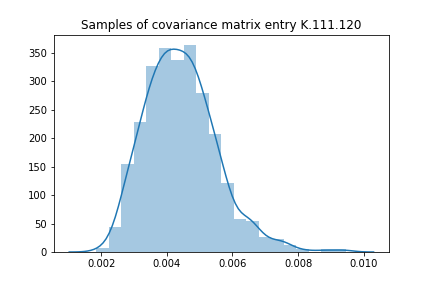
\includegraphics[width=\textwidth]{img/07_0/K_111_120_samples.png}
		\caption{The entry 111/120 of the covariance matrix of the GPLVM model trained on a dataset of $N=120$, $D=754$. For this covariance entry, the algorithm has converged sufficiently and sufficiently fast.}
		\label{fig:K_111_120_gplvm}
	\end{subfigure}
	\begin{subfigure}[b]{0.4\textwidth}
		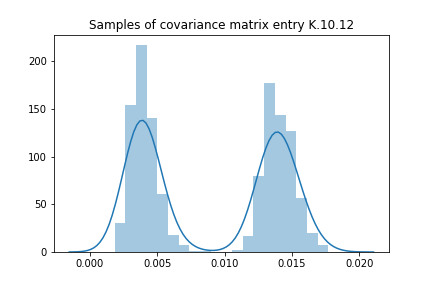
\includegraphics[width=\textwidth]{img/07_0/K_10_12_samples.png}
		\caption{The entry 10/12 of the covariance matrix of the GPLVM model trained on a dataset of $N=120$, $D=754$. For this covariance entry, the algorithm has not converged sufficiently or sufficiently fast.}
		\label{fig:K_10_12_gplvm}
	\end{subfigure}
	\caption{}
	\label{fig:cov_entries_gplvm}
\end{figure}
The plots in \ref{fig:cov_entries_gplvm} show the distribution sampled by the variational inference algorithm as kde and histogram plot of two entries of the covariance matrix. The ratio of sampled values in the main peak compared to the other peaks, as well as the position of the global maximum of this distribution compared to the effectively used value, which is the overall mean and further on used quantity, give a good estimate of the error that is effecting the further results for a calculation where the ELBO has converged. Entry K.10.12, figure \ref{fig:K_10_12_gplvm}, shows critical behavior where the algorithm probably has not converged sufficiently, or where different values seem to provide stable solutions. This is especially interesting, since time-dependent solutions to the covariance between two stocks seem like a viable alternative. The entry K.111.120, figure \ref{fig:K_111_120_gplvm} instead provides a clearer image of what was expected, where the mean is closer to the maximum of probability mass. The learning equation,
\begin{equation}%GPLVM Learning Equation
	\hat{Y}_{GPLVM} = K [(K+\delta_{ij}\sigma_{n})Y],
	\label{eq:GPLVM_learning_equation}
\end{equation}
is used to calculate predictions from the model. Testing the prediction power of models is usually done in several steps, where the first step is to test it against predicting the initial data. With the predictions, we can calculate errors based on the model reproducing the dataset it was trained on, resulting in $\hat{Y}$, a matrix of equal size as $Y$. Since the model includes uncertainty and noise, we do not expect a perfect reconstruction of the data fed into the model. Comparing the data with the predictions yields interesting insight, since several possible errors can be directly visible from these results. But first, it is necessary to discuss various ways of quantifying the quality of a model. The Evidence Lower Bound, which was introduced in chapter \ref{sec:bayes}, is a unit-less measure of the quality of a model. The higher the ELBO, the better the results. Comparing the ELBO values gives insight into how good a model was able to reproduce the true posterior with the variational inference distribution approximation of the true posterior, using KL-Divergence. The initial expectation is that models with more dimensions taken into account in the latent space (higher values of Q) perform better, and how more sophisticated kernels outperform less sophisticated kernels like the linear kernel \cite{Nirwan_2019}. As another measure of performance, the $R^2$ values of the models are calculated and plotted in the same fashion as the ELBO values. These are calculated of the data and predictions using the \textit{LinearRegression} model from \textit{arviz} \cite{arviz_2019}, which uses the regular definition of the coefficient of determination ($R^2$). 
\begin{equation}%Coefficient of Determination R^2
	R^2 = 1 - \frac{\sum (Y-\hat{Y})^2}{\sum (Y-\bar{Y})^2}
	\label{eq: GPLVM R^2 calculation}
\end{equation}
The coefficient of determination is a measure of how well the model has reconstructed the predictions as a function of the data, but it still has missing information. If we plot the data points against the corresponding predictions, we would expect a single straight line with slope 1 and intercept 0 for a perfect result. Since the model incorporates noise, we still would expect the model to have a slight deviation from this line, but it should be centered around the line. If the deviation is centered around the line, a Huber regression fit through the data-prediction pairs would also have a slope of 1 and an intercept of 0.  Huber regression was chosen over linear regression, due to the outliers in predictions only accounting linearly instead of quadratic when doing linear least squares optimization during regression, and therefore provided much more stable and reliable information about the intercept and slope values. For more information, see Appendix \ref{sec:huber_reg}. While reconstructing the model initially tested against these kind of data in \cite{Nirwan_2019}, the plots showed an abnormality.
\begin{figure}%CENTRAL IMAGE with problem statement of Y-Y_hat pairs reflecting problem.
	\centering
	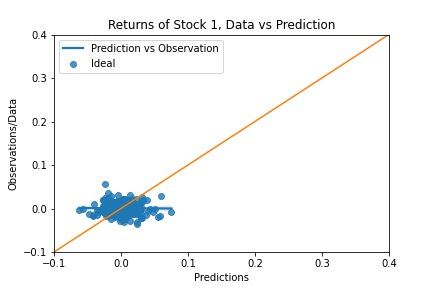
\includegraphics[width=4in]{img/07_0/problem.jpg}
	\caption[Data-Prediction Plot GPLVM]
	{An example of a Y-$\hat{Y}$-pair plot of a stock fit with a Stochastic Process Latent Variable Model. A linear least squares fit is added, highlighting the observed effect of the predictions not accurately reflecting the data. Predictions on a regular basis seem to underestimate comparably high returns, and overestimate comparably low returns, resulting in a slope of the linear fit that is way off of the expectation.}
	\label{fig:gplvm_pair_plot_central}
\end{figure}
The model at hand overestimates lower returns, and underestimate higher returns, resulting in non-optimal ELBO and $R^2$ values. Higher ELBO values represent better estimation of the true posterior, but are not able to be interpreted with a higher bound due to the nature of the KL-divergence. $R^2$ values, the coefficients of determination, are a measure of the prediction quality, as a numerical value of how similar data and predictions are. A value relatively close to one is optimal, but due to the nature of how noisy stock market data is, a value of 1 would not be desirable. Because then the model would have learned a lot of noise as feature. Models that show considerably lower values in ELBO compared to the respective other models sharing characteristics probably have not converged towards the optimal point on the energy landscape, for example $Q=3$ and $Q=6$ with the exponential kernel in figure \ref{fig:gplvm_ELBO_R2}. 
\begin{figure}
	\centering
	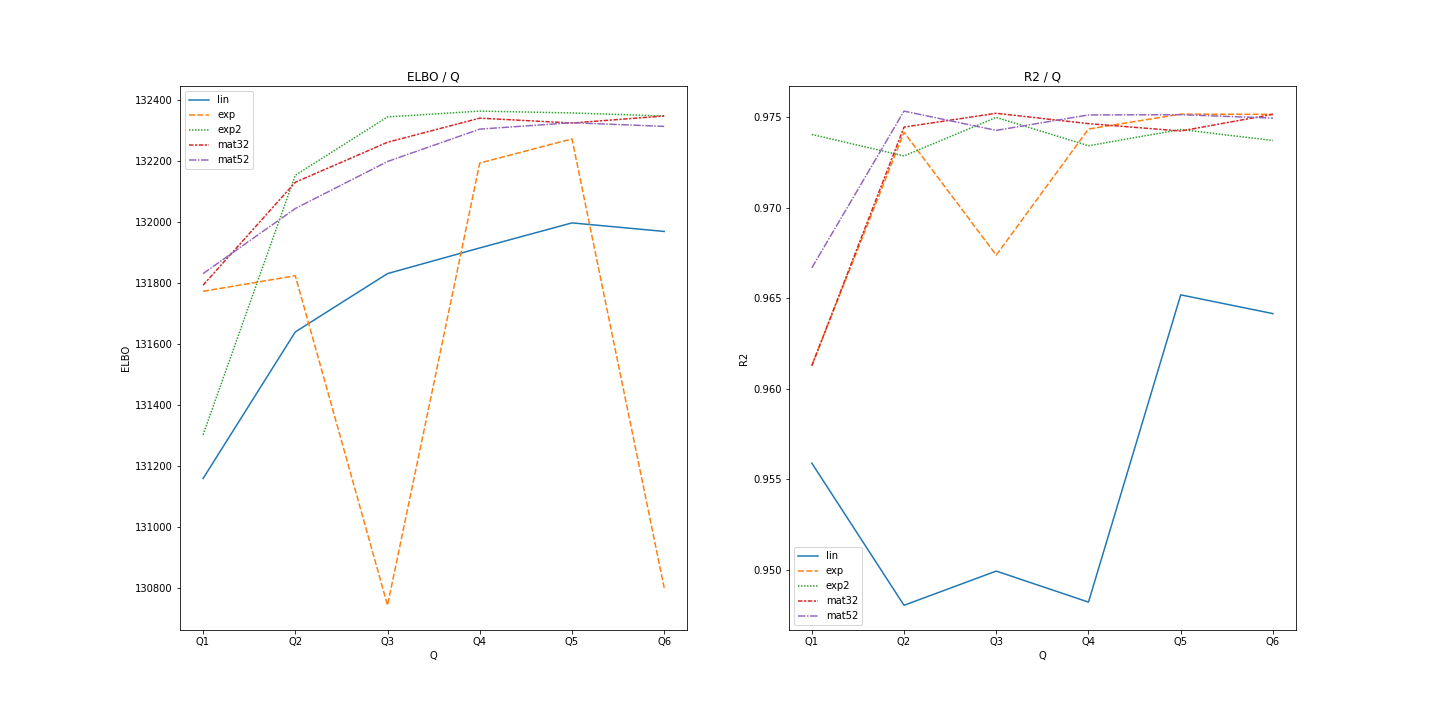
\includegraphics[width=7in]{img/07_0/modelGPLVM_Qs.png}
	\caption[ELBO and $R^2$ comparison for the GPLVM model]{ELBO and $R^2$ values for the GPLVM model and $N=60$, $D=754$. }
	\label{fig:gplvm_ELBO_R2}
\end{figure}
We can find another metric of model quality in the distribution and mean values of intercepts, as well as slope values. These distributions show how the model has predicted the slopes, figure \ref{fig:gplvm_slopes}, and intercepts, figure \ref{fig:gplvm_intercepts}, of all stocks entailed in the data matrix. Experiments show good agreement with expectations for the slopes, since they are close to the expected value of 1. Still they remain mostly to the left side of the bar at slope$=1$, coinciding with the expectation that a model can never learn everything about a naturally noisy system. The distributions of the intercepts should be centered around the vertical line at intercept$=0$, which would imply that almost the same number of stocks are over predicted as are under predicted.
\begin{figure}%Intercept distributions
	\centering
	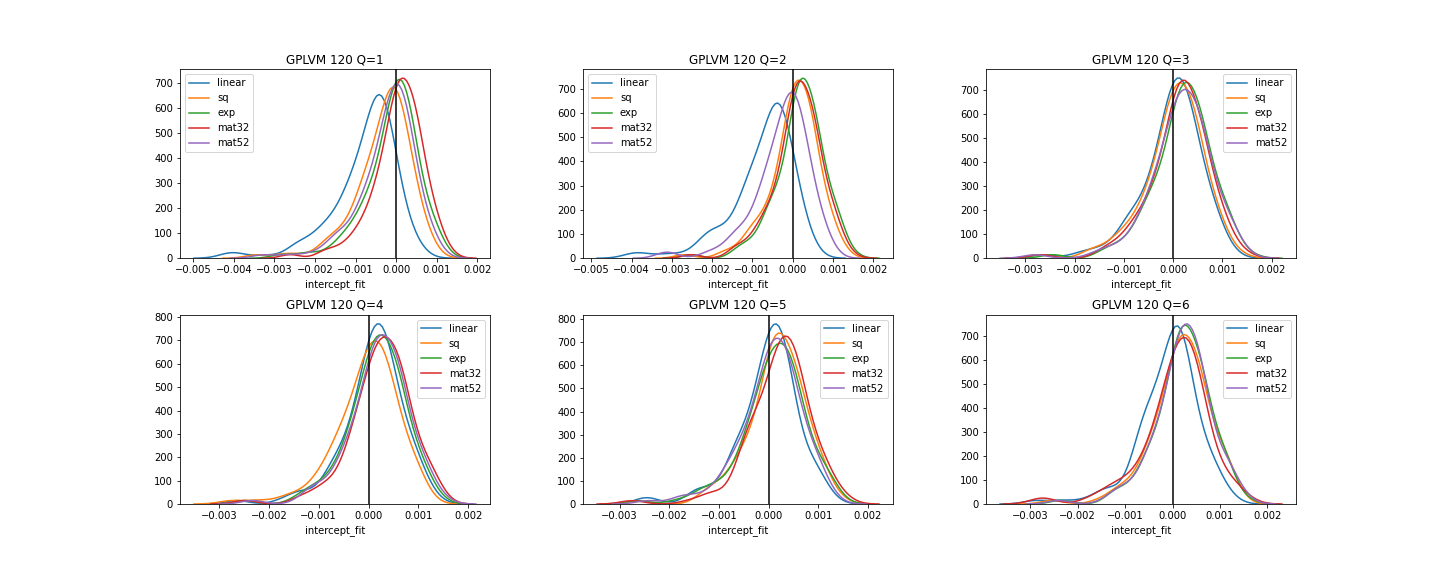
\includegraphics[width=7in]{img/07_0/intercept_fit_gplvm_120.png}
	\caption[Intercept Distributions for GPLVM]{Comparing the distributions of stock slope values from the GPLVM model with different kernel functions over the scope of all latent dimensions. }
	\label{fig:gplvm_intercepts}
\end{figure}
\begin{figure}%Slope distributions
	\centering
	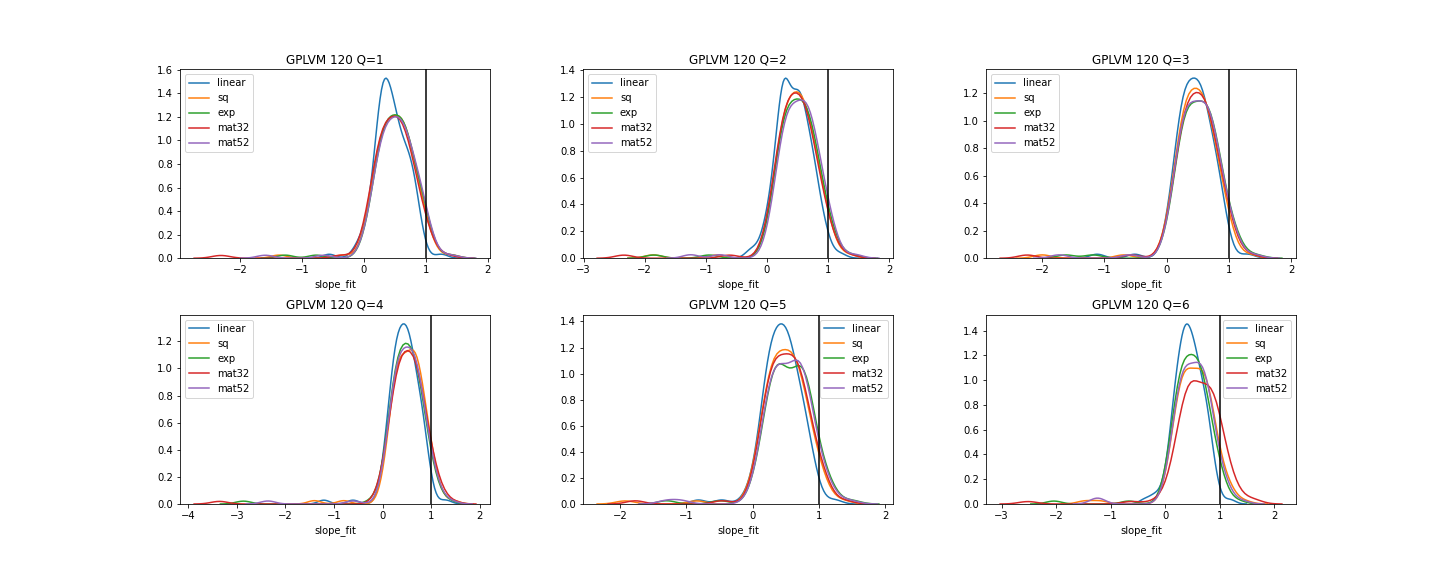
\includegraphics[width=7in]{img/07_0/slope_fit_gplvm_120.png}
	\caption[Slope distributions for GPLVM]
	{Comparing the intercept values of the GPLVM model with different kernel functions over the scope of all latent dimensions. }
	\label{fig:gplvm_slopes}
\end{figure}
\newline \newline
Several sanity checks for the model are displayed, where the distributions of the samples, or just the distributions of the values of the entries of the vector-like or matrix-like objects are plotted. Within these checks, larger samples of outliers can be detected, that may stem from local minima in the energy landscape in the variational inference solver. 
\begin{figure}%fig:gplvm_noises   Observation noise distribution sanity checks
	\centering
	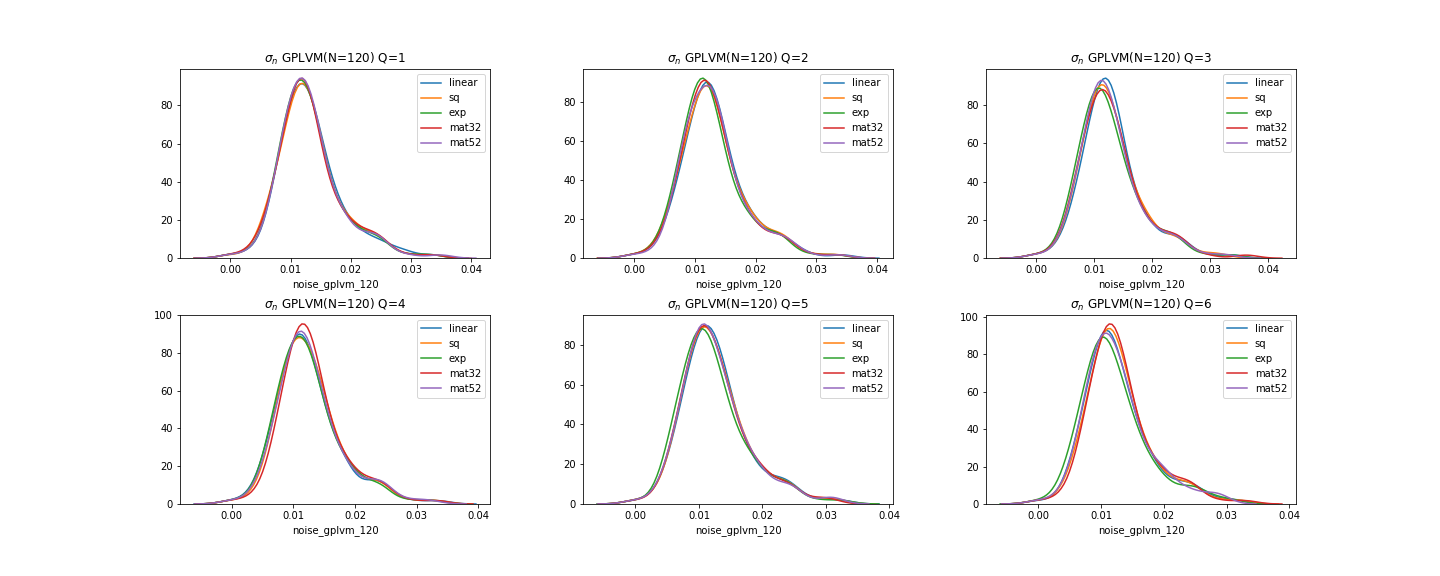
\includegraphics[width=7in]{img/07_0/noise_GPLVM_120.png}
	\caption[Signal Noise distributions GPLVM]
	{Distributions of vector elements of $\sigma_n$. The closer values are to 0, the more accurate the measurements are according to the model. The observation noise is non-isotropic.}
	\label{fig:gplvm_noises}
\end{figure}
Figure \ref{fig:gplvm_noises}, together with the learning equation, gives a direct interpretation of the kernel noise as the observation noise, since it is added to the diagonal of the covariance matrix. These entries resemble the self-correlation of the stocks. Also, it is necessary to point out, that these kernel density estimate plots of the variables can be misleading, since e.g. the noise is restricted to $\mathbb{R}_0^+$, since noise can not improve the measurement accuracy to be better than perfect.
\begin{figure}%fig:gplvm_variances     Variance noise distribution sanity checks ~ volatility per stock
	\centering
	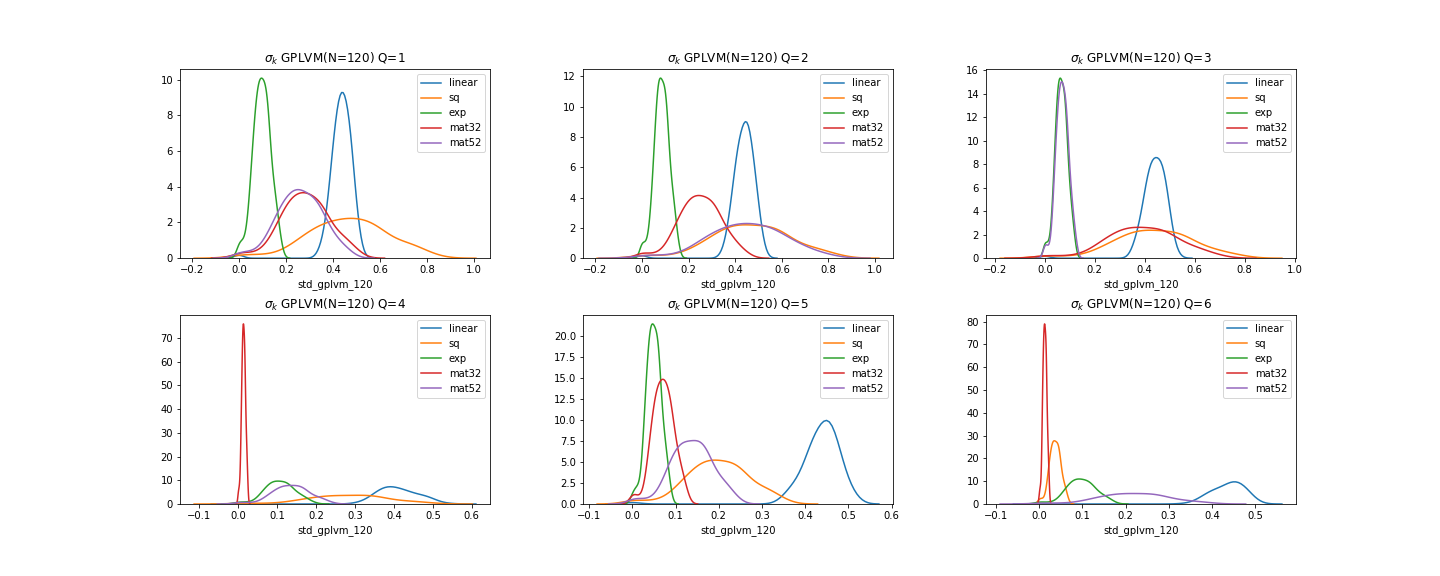
\includegraphics[width=7in]{img/07_0/std_GPLVM_120.png}
	\caption[Standard Deviation Distributions GPLVM]
	{Distributions of vector elements of $\sigma_k$. These values represent volatility in a financial context.}
	\label{fig:gplvm_variances}
\end{figure}
In figure \ref{fig:gplvm_variances} the variances are shown. These are estimated once for each stock, and then kept constant over time. The linear kernel is observed to more often need a higher volatility to function, even though it was outperformed by the other kernels. \newline
Similarly, the entries of the inferred covariance matrix entries' distribution can be plotted, like in figure \ref{fig:gplvm_covariances}. They resemble the statistical connection between two stocks, and should also be $\in\mathbb{R}_0^+$. This is due to covariance matrices, by definition, being positive semi-definite. Also having many entries $>1$ seems improbable, since that would imply a covariance of very great degree, in turn implying a correlation of an unusually high degree. A very large part of the values is close to 0, implying a sane model. 
\begin{figure}%Covariance matrices sanity checks
	\centering
	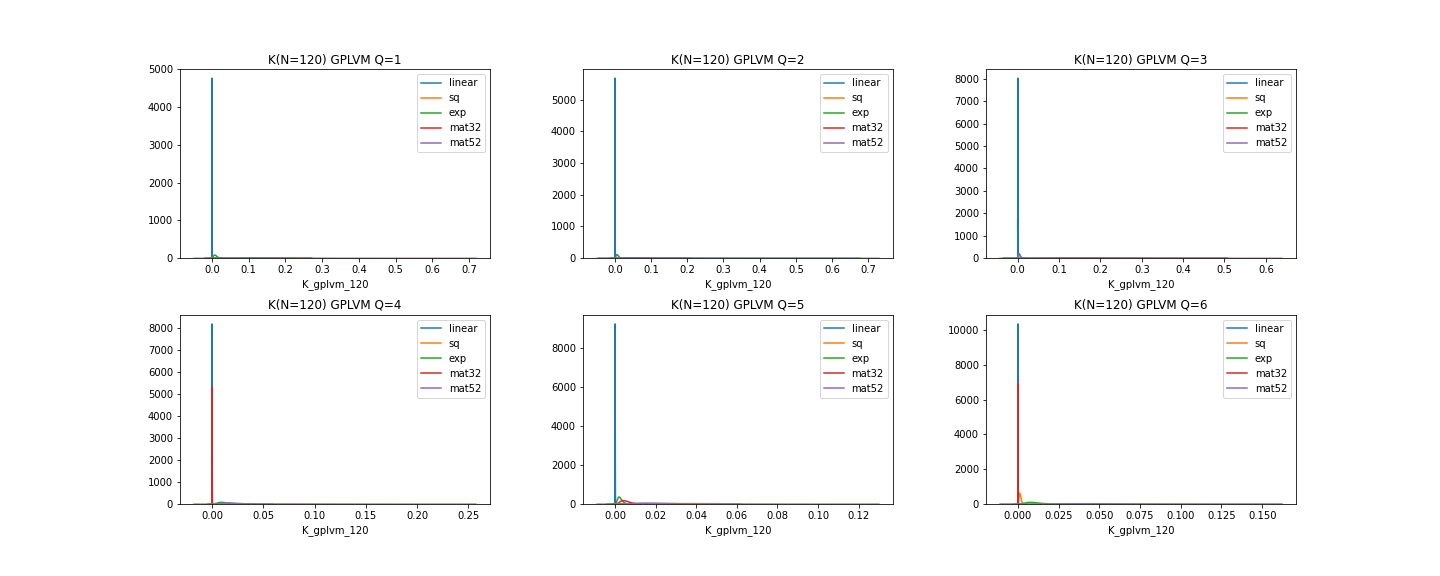
\includegraphics[width=7in]{img/07_0/K_GPLVM_120.png}
	\caption[Covariance Matrix Entry Distributions GPLVM]
	{Distributions of the values of the entries of the covariance matrices. }
	\label{fig:gplvm_covariances}
\end{figure}
After considering the sanity of the model compared to the expectations that can be deduced from observations of reality, different hypotheses can be formulated to explain the deviance from the expectation in the data-prediction-pair plot \ref{fig:gplvm_pair_plot_central}. At first, the effects of the size of the data matrices used to train the model were considered. For this, the size of the data matrix was scaled to include data matrices with different numbers of stocks, and different time periods over which the observations have taken place. We therefore look at different types of flaunty behaviour in the reconstruction, comparing figures \ref{fig:gplvm_N20_pairs}, \ref{fig:gplvm_N60_pairs}, \ref{fig:gplvm_N100_pairs} and \ref{fig:gplvm_N120_pairs}, which show typical behaviour of data-prediction pair plots for $N=20$ \ref{fig:gplvm_N20_pairs}, $N=60$ \ref{fig:gplvm_N60_pairs}, $N=100$ \ref{fig:gplvm_N100_pairs}, and $N=120$ \ref{fig:gplvm_N120_pairs}. 
\begin{figure}%fig:gplvm_N20_pairs
	\centering
	\begin{subfigure}[l]{0.3\textwidth}
		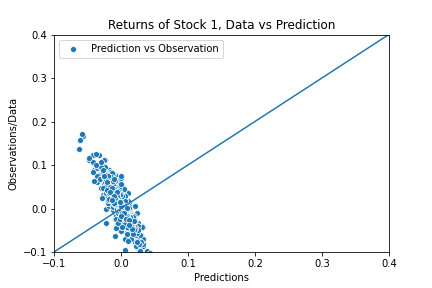
\includegraphics[width=\textwidth]{img/07_0/N20/Q3_kernel3_stock1_scatter.png}
	\end{subfigure}
	\begin{subfigure}[c]{0.3\textwidth}
		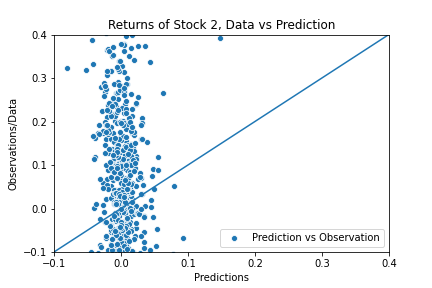
\includegraphics[width=\textwidth]{img/07_0/N20/Q3_kernel3_stock2_scatter.png}
	\end{subfigure}
	\begin{subfigure}[r]{0.3\textwidth}
		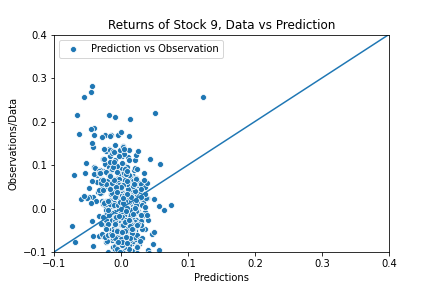
\includegraphics[width=\textwidth]{img/07_0/N20/Q3_kernel3_stock9_scatter.png}
	\end{subfigure}
	\caption[Y-$\hat{Y}$ pair plots for N=20 with the GPLVM model]{Plots from the GPLVM reconstruction with the $N=20$, $D=754$ dataset. The reconstruction failed, but the model had a fast convergence in distributions. }
	\label{fig:gplvm_N20_pairs}
\end{figure}
\begin{figure}%fig:gplvm_N60_pairs
	\centering
	\begin{subfigure}[l]{0.3\textwidth}
		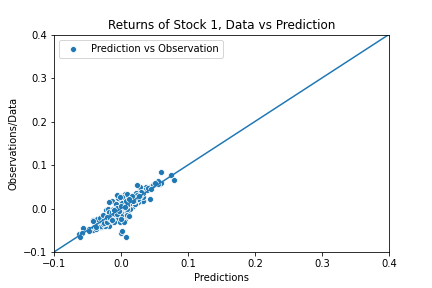
\includegraphics[width=\textwidth]{img/07_0/N60/Q1_kernel1_stock1_scatter.png}
	\end{subfigure}
	\begin{subfigure}[c]{0.3\textwidth}
		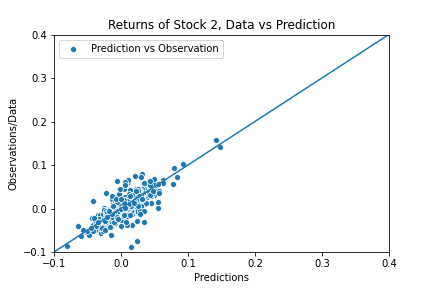
\includegraphics[width=\textwidth]{img/07_0/N60/Q1_kernel1_stock2_scatter.png}
	\end{subfigure}
	\begin{subfigure}[r]{0.3\textwidth}
		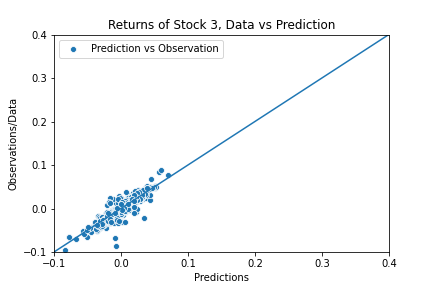
\includegraphics[width=\textwidth]{img/07_0/N60/Q1_kernel1_stock3_scatter.png}
	\end{subfigure}
	\caption[Y-$\hat{Y}$ pair plots for N=60 with the GPLVM model]{Plots from the GPLVM reconstruction with the $N=60$, $D=754$ dataset. The reconstruction worked properly. }
	\label{fig:gplvm_N60_pairs}
\end{figure}
\begin{figure}%fig:gplvm_N100_pairs
	\centering
	\begin{subfigure}[l]{0.3\textwidth}
		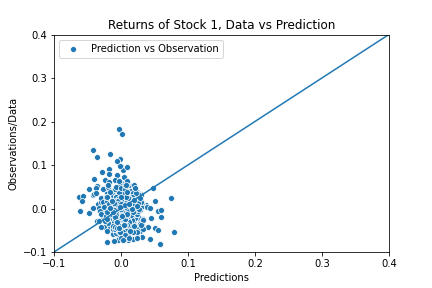
\includegraphics[width=\textwidth]{img/07_0/N100/Q1_kernel1_stock1_scatter.png}
	\end{subfigure}
	\begin{subfigure}[c]{0.3\textwidth}
		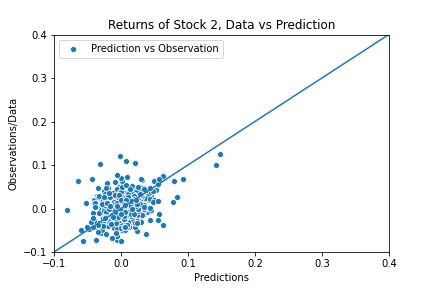
\includegraphics[width=\textwidth]{img/07_0/N100/Q1_kernel1_stock2_scatter.png}
	\end{subfigure}
	\begin{subfigure}[r]{0.3\textwidth}
		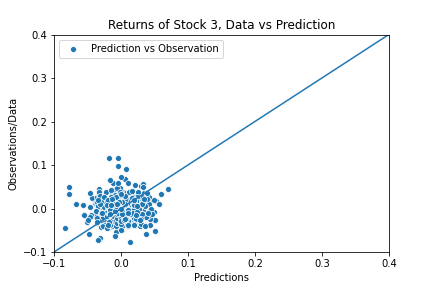
\includegraphics[width=\textwidth]{img/07_0/N100/Q1_kernel1_stock3_scatter.png}
	\end{subfigure}
	\caption[Y-$\hat{Y}$ pair plots for N=100 with the GPLVM model]{Plots from the GPLVM reconstruction with the $N=60$, $D=754$ dataset. The circular shape of the cloud indicates that the distributions of $Y$ and $\hat{Y}$ are well fit, but subpar reconstruction.}
	\label{fig:gplvm_N100_pairs}
\end{figure}
\begin{figure}%fig:gplvm_N120_pairs
	\centering
	\begin{subfigure}[l]{0.3\textwidth}
		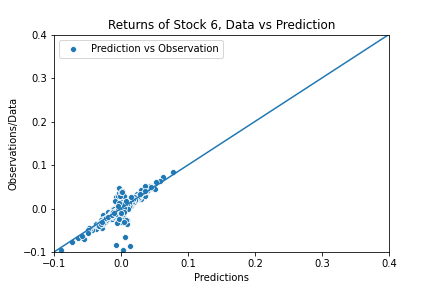
\includegraphics[width=\textwidth]{img/07_0/N120/Q1_kernel3_stock6_scatter.png}
	\end{subfigure}
	\begin{subfigure}[c]{0.3\textwidth}
		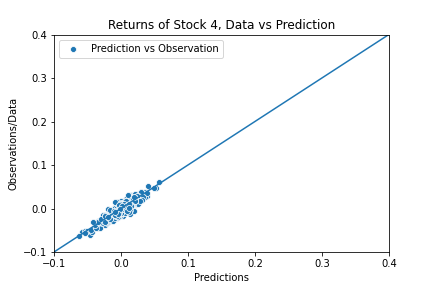
\includegraphics[width=\textwidth]{img/07_0/N120/Q6_kernel1_stock4_scatter.png}
	\end{subfigure}
	\begin{subfigure}[r]{0.3\textwidth}
		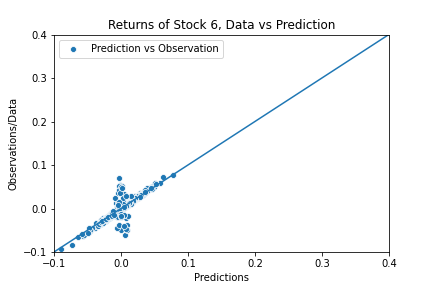
\includegraphics[width=\textwidth]{img/07_0/N120/Q3_kernel5_stock6_scatter.png}
	\end{subfigure}
	\caption[Y-$\hat{Y}$ pair plots for N=120 with the GPLVM model]{Plots from the GPLVM reconstruction with the $N=60$, $D=754$ dataset. We can find a good estimation of the true posterior, and a good reconstruction, but also find that in some cases, to match the data distribution some predictions are very close to 0, not representing the data at all.}
	\label{fig:gplvm_N120_pairs}
\end{figure} 
From this we can conclude, that the model has an intrinsic error reconstructing the covariance structure while still matching the target 1D-distributions of the data. In the following part of this chapter, different possible solutions to this problem are discussed. 
%%
%VOLATILITY CORRECTED GPLVM
%%
\subsection{Volatility normalized datasets}
Since the GPLVM model does not have time dependent volatility, different possible scenarios can not be incorporated into the model. For example, stocks with comparably high, but also highly varying volatility will not be represented very well, since the model will probably infer the mean volatility for this value. Therefore, the model was also tested against datasets where the stocks were normalized (VN - Volatility normalized) one by one, using the inferred volatility of a HCMC optimized GARCH process, compare sections \ref{sec:arch} and \ref{sec:mcmc}, as well as \cite{pyflux}. The results are again depicted through example pictures of the systematic deviation observed in the $Y-\hat{Y}$-pair plots. Also, sanity checks were performed, e.g. plotting noises and variances. Here, since the expected volatility was used to normalize the returns on their respective predicted volatilities, the variance in figure \ref{fig:variance_vcr} should be close to zero. This aspect was recognized correctly by the model. The inherent noise should be small, and is shown in \ref{fig:noise_vcr}. These figures also show, that the calculation does not resemble correctly our expectations of the model. Also, we acknowledge that another prior distribution would have been a better suited choice, since the kernel density estimate plots show values smaller than 0, which are forbidden through the generating process chosen. 
\begin{figure}[h!]
	\centering
	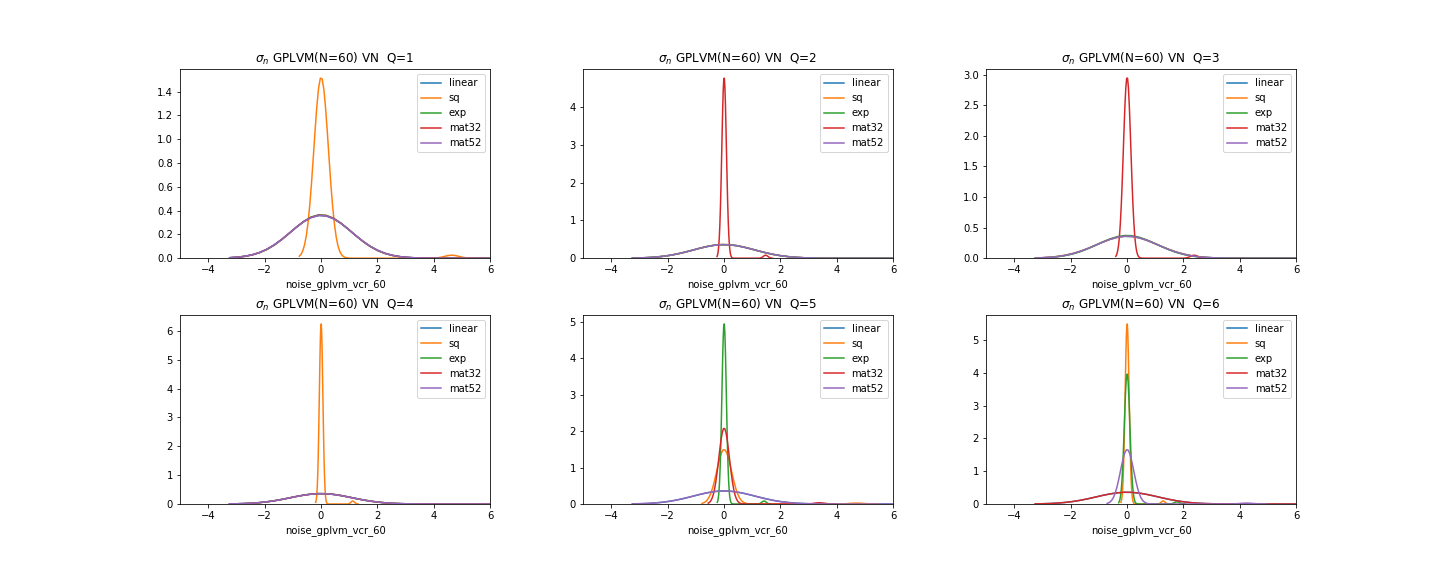
\includegraphics[width=7in]{img/07_0/noise_GPLVM_vcr_60.png}
	\caption[Noise Distribution of GPLVM with VCR dataset]{Distributions of $\sigma_{n}$, which were trained on a VN dataset with $N=60$ and $D=125$.}
	\label{fig:noise_vcr}
\end{figure}
\begin{figure}[h!]%fig:noise_variance_vcr
	\centering
	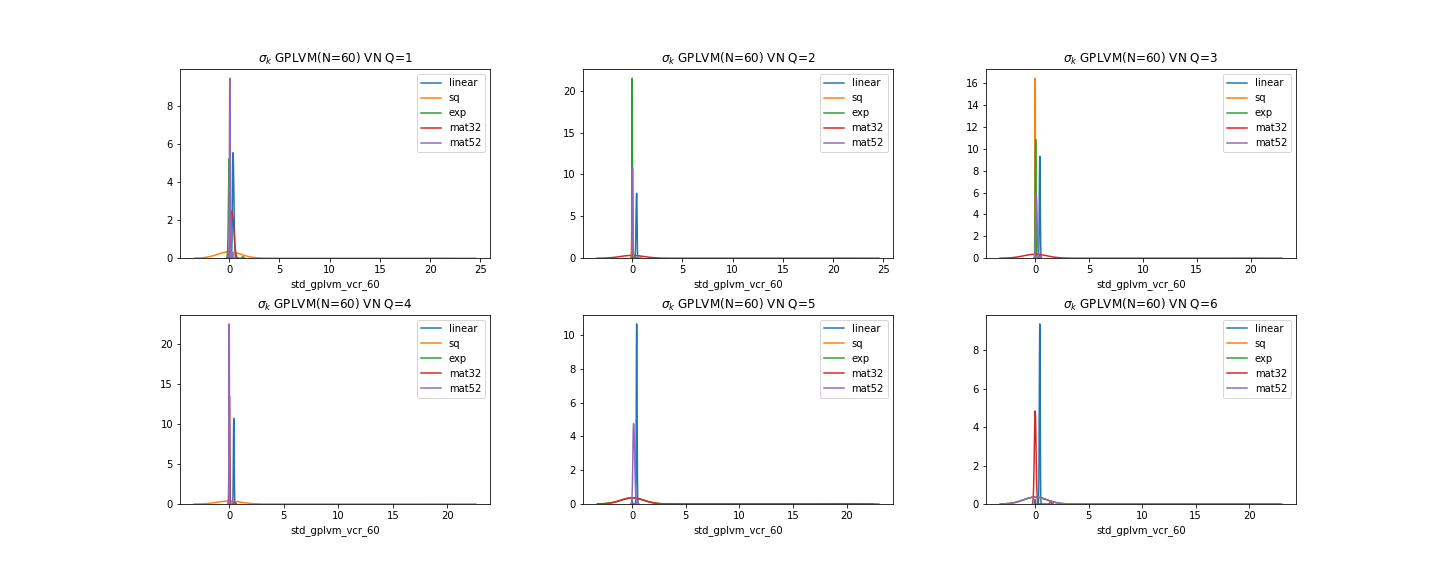
\includegraphics[width=7in]{img/07_0/std_GPLVM_vcr_60.png}
	\caption[Variance Distributions of GPLVM with VN dataset]{Distributions of $\sigma_{n}$, which were trained on a VN dataset with $N=60$ and $D=125$.}
	\label{fig:variance_vcr}
\end{figure}
Since we found a dependency on the size of the data matrix $Y$, we test the model with different sizes of datasets, shown in figure \ref{fig:dataset_size_init}. We recorded which sizes of data sets, within the confinement of the largest data set of $N=120$ and $D=754$, would successfully run without stan rejecting the initial values due to bad conditioning. Stan uses several hundreds of initial values for initialization. An orange dot is used if the model did not initialize. If the model did initialize, a blue dot is used. All experiments were carried out using a squared exponential kernel and using $Q=3$ latent dimensions.
\begin{figure}[h!]%Initializable Y-sizes with the GARCH-volatility-corrected dataset sizes. 
	\centering
	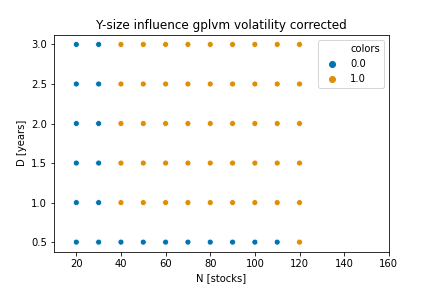
\includegraphics[width=4in]{img/07_0/size_influence-gplvm_vcr.png}
	\caption[Initialization of GPLVM model VN datasets]
	{Shown here, in the same style as with the regular datasets and the GPLVM-model is the influence of dataset sizes on initialization. Again, blue points represent input matrix sizes, that were successfully initialized, while orange points represent matrix sizes, where initialization failed.}
	\label{fig:dataset_size_init}
\end{figure}
We observe that the data sets that initialized successfully were either over very short time frames, or with very little stocks. We conclude therefore, that the used GARCH process breaks down for longer time frames due to errors propagating, as well as for more observed stocks, which reflect a more complicated part of the true covariance structure. In comparison, experiments showed that the regular, unnormalized, data set always initialized properly. \newline \newline
The example data set evaluated was $N=60$, $D=125$. It showed a range of behaviors when reproducing the data. Examples of these behaviors are shown in figures \ref{fig:gplvm_vcr_pairs}, where the model does a very good fit (\textit{left}), reproduces a very bad fit (\textit{center}), and shows the property to reproduce a correct target distribution but not with the right data points (\textit{right}). These pitfalls have also been seen before, in the GPLVM model, especially figures \ref{fig:gplvm_N20_pairs}, \ref{fig:gplvm_N100_pairs}, and \ref{fig:gplvm_N120_pairs}. The suspicion therefore arises, that normalizing the dataset either went wrong, or destroyed the overall covariance structure in such a way, that the model could not reconstruct it. 
\begin{figure}%fig:gplvm_N120_pairs
	\centering
	\begin{subfigure}[l]{0.2\textwidth}
		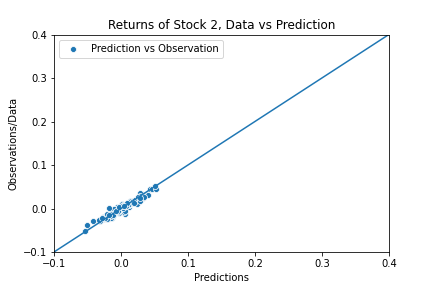
\includegraphics[width=\textwidth]{img/07_0/N60D123/Q1_kernel1_stock2_scatter.png}
	\end{subfigure}
	\begin{subfigure}[c]{0.3\textwidth}
		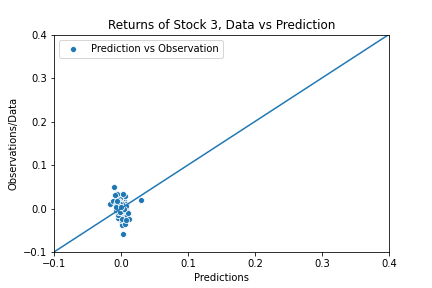
\includegraphics[width=\textwidth]{img/07_0/N60D123/Q1_kernel1_stock3_scatter.png}
	\end{subfigure}
	\begin{subfigure}[r]{0.3\textwidth}
		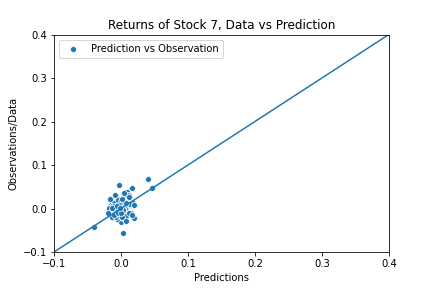
\includegraphics[width=\textwidth]{img/07_0/N60D123/Q1_kernel1_stock7_scatter.png}
	\end{subfigure}
	\caption[Y-$\hat{Y}$ pair plots for $N=60$, $D=125$ VN-data with the GPLVM model]{Plots from the GPLVM reconstruction with the $N=60$, $D=754$ dataset. We can find a good estimation of the true posterior, and a good reconstruction, but also find that in some cases, to match the data distribution some predictions are very close to 0, not representing the data at all.}
	\label{fig:gplvm_vcr_pairs}
\end{figure}